\documentclass[a4paper]{scrartcl}


\usepackage[utf8]{inputenc}
\usepackage[ngerman]{babel}
\usepackage{enumerate}
\usepackage{tikz}
\usepackage{fancyhdr}
\usepackage{lastpage}
\usepackage{verbatim}

\usepackage{listings}
\setlength{\parindent}{0mm}
\usepackage{graphicx}
\usepackage{amsmath}
\usepackage{algorithm2e}

\pagestyle{fancy}
\fancyhead[L]{SS 2017\\Joshua Hartmann}
\fancyhead[C]{Entwurf und Synthese von Eingebetteten Systemen\\Manfred Opel}
\fancyhead[R]{Blatt 9\\Nicola Staller}

\fancyfoot[L]{}
\fancyfoot[C]{\thepage /\pageref{LastPage}}
\fancyfoot[R]{}

\renewcommand{\textheight}{700px}
\renewcommand{\footskip}{10px}
\newcommand*\xor{\mathbin{\oplus}}
\begin{document}	
\section*{Aufgabe 1: High Level Synthese: Hu- und List-Scheduling}

\begin{enumerate}[(a)]
	\item Die NOPs sind jeweils nur angedeutet um die Übersichtlichkeit zu verbessern.
	
	ASAP:\\	
	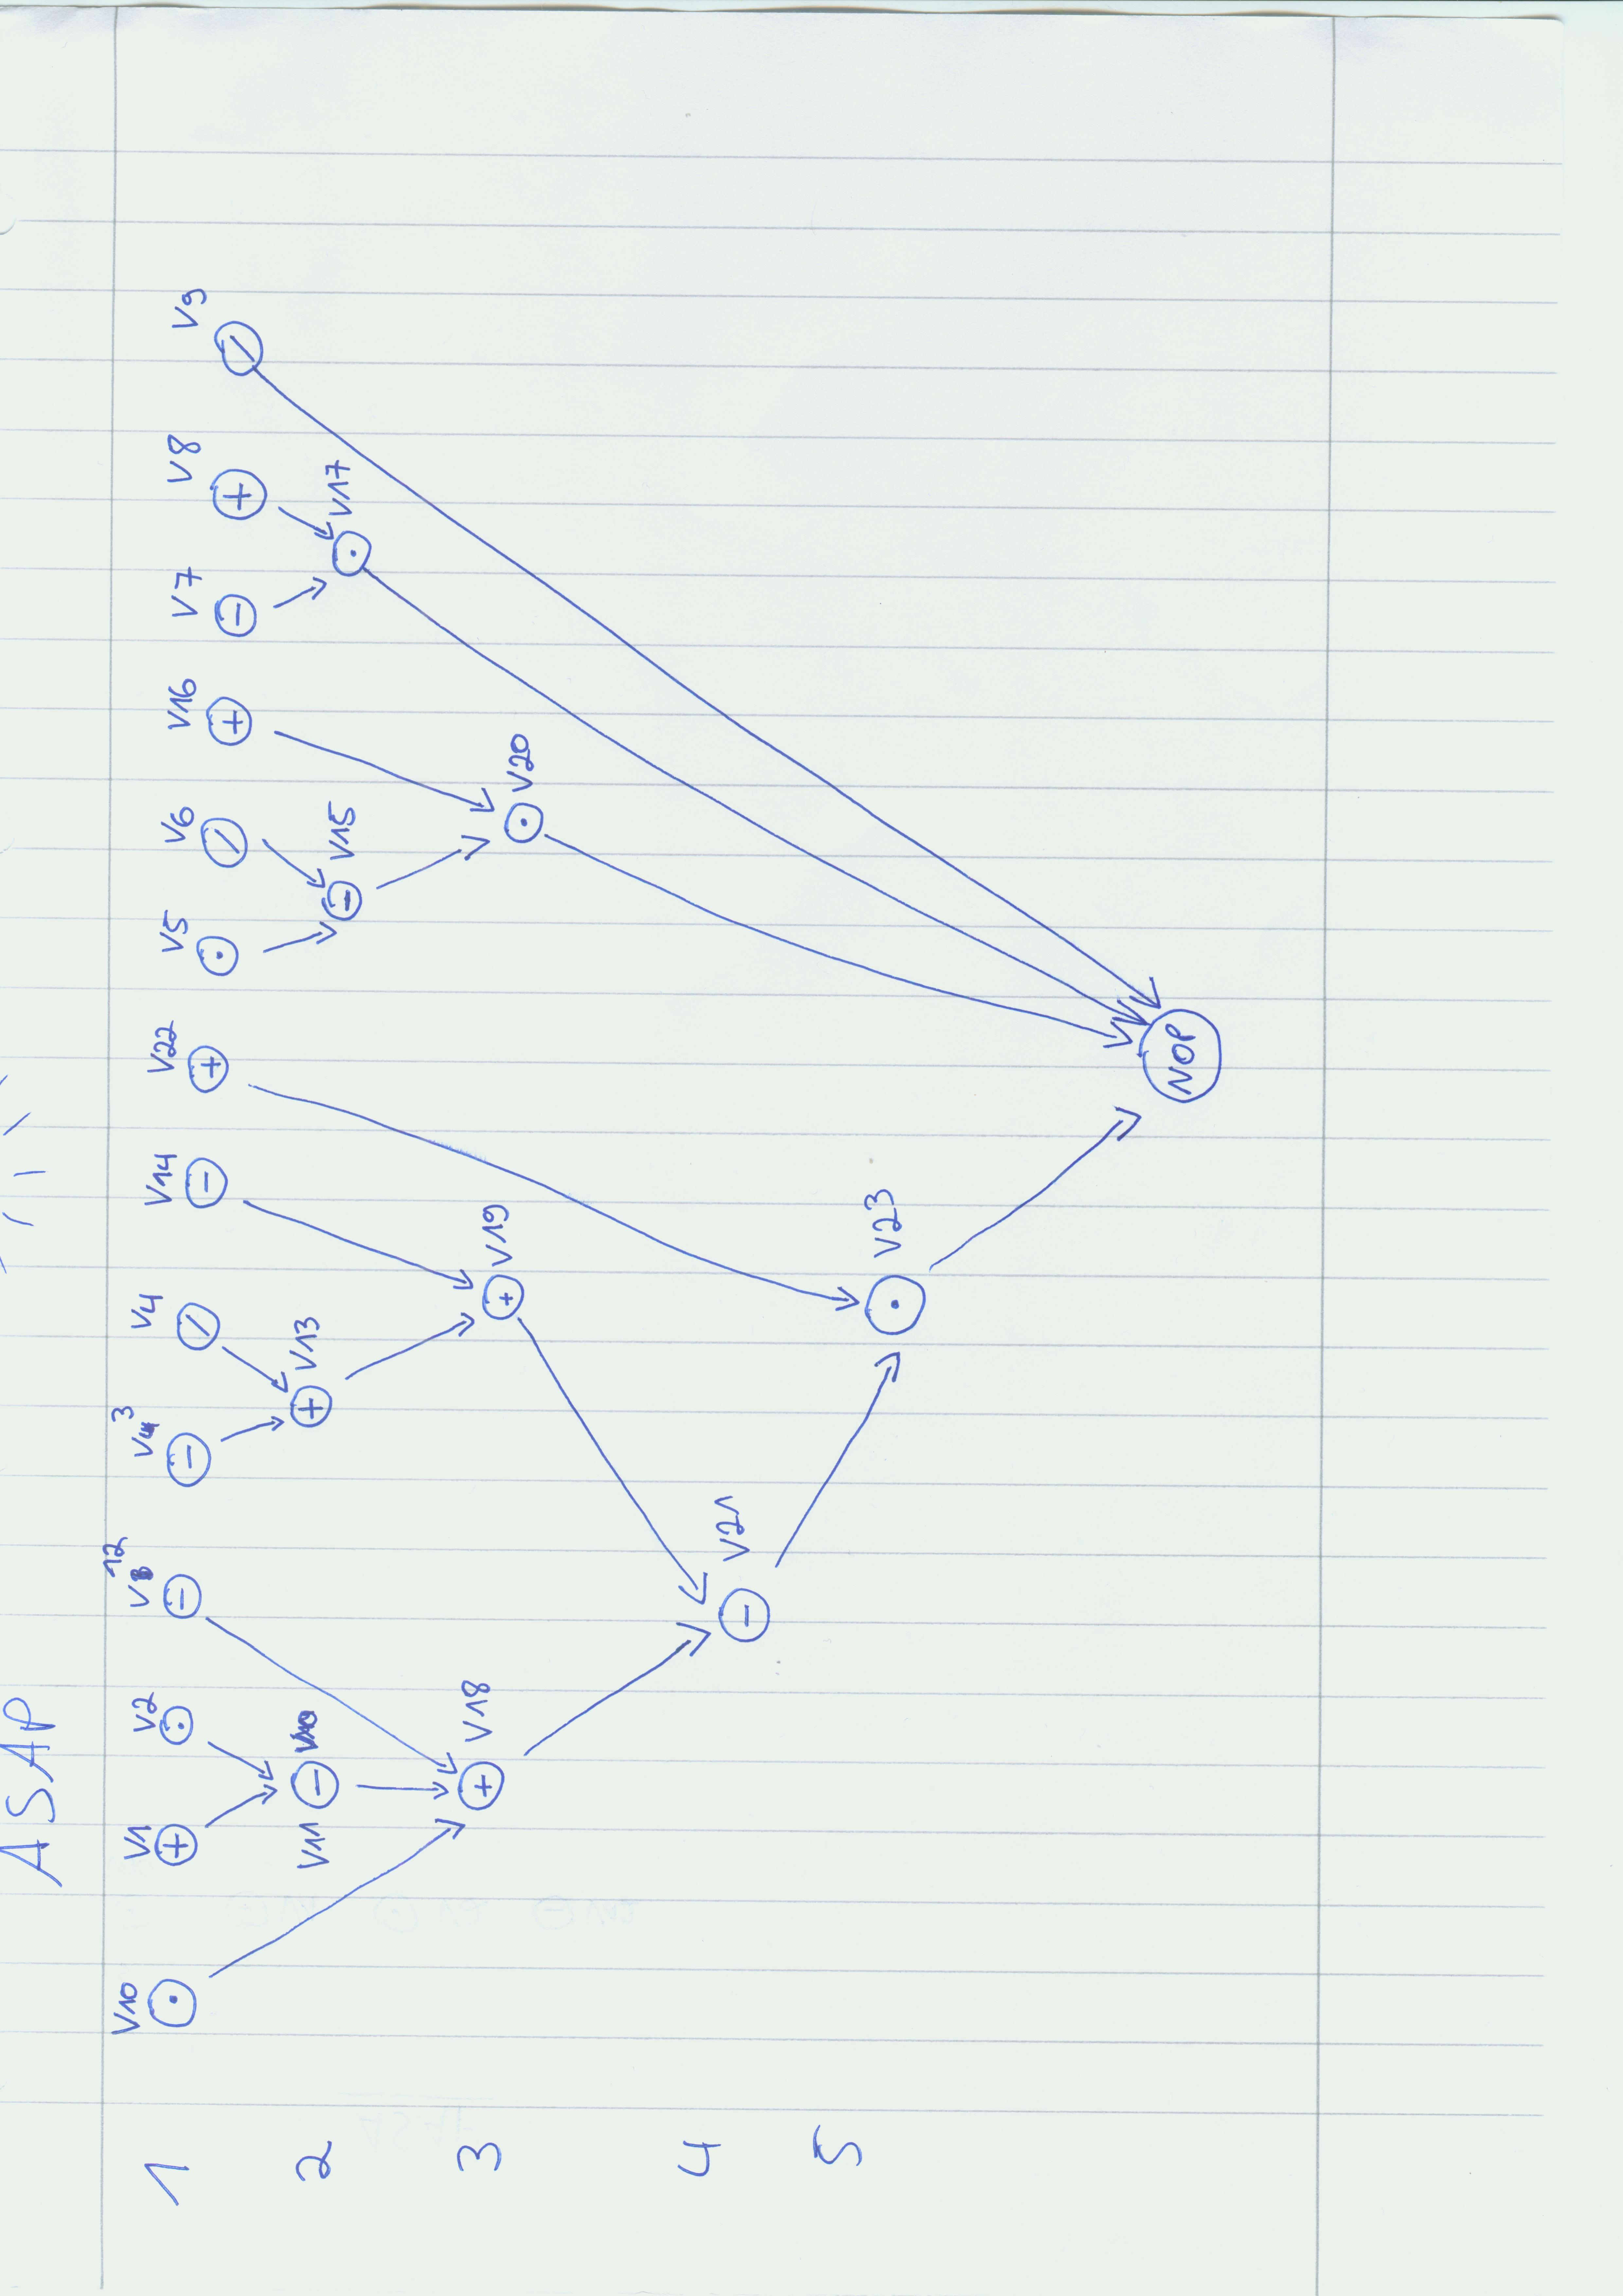
\includegraphics[scale=0.5, angle = -90]{Image124}
	
	ALAP:\\	
	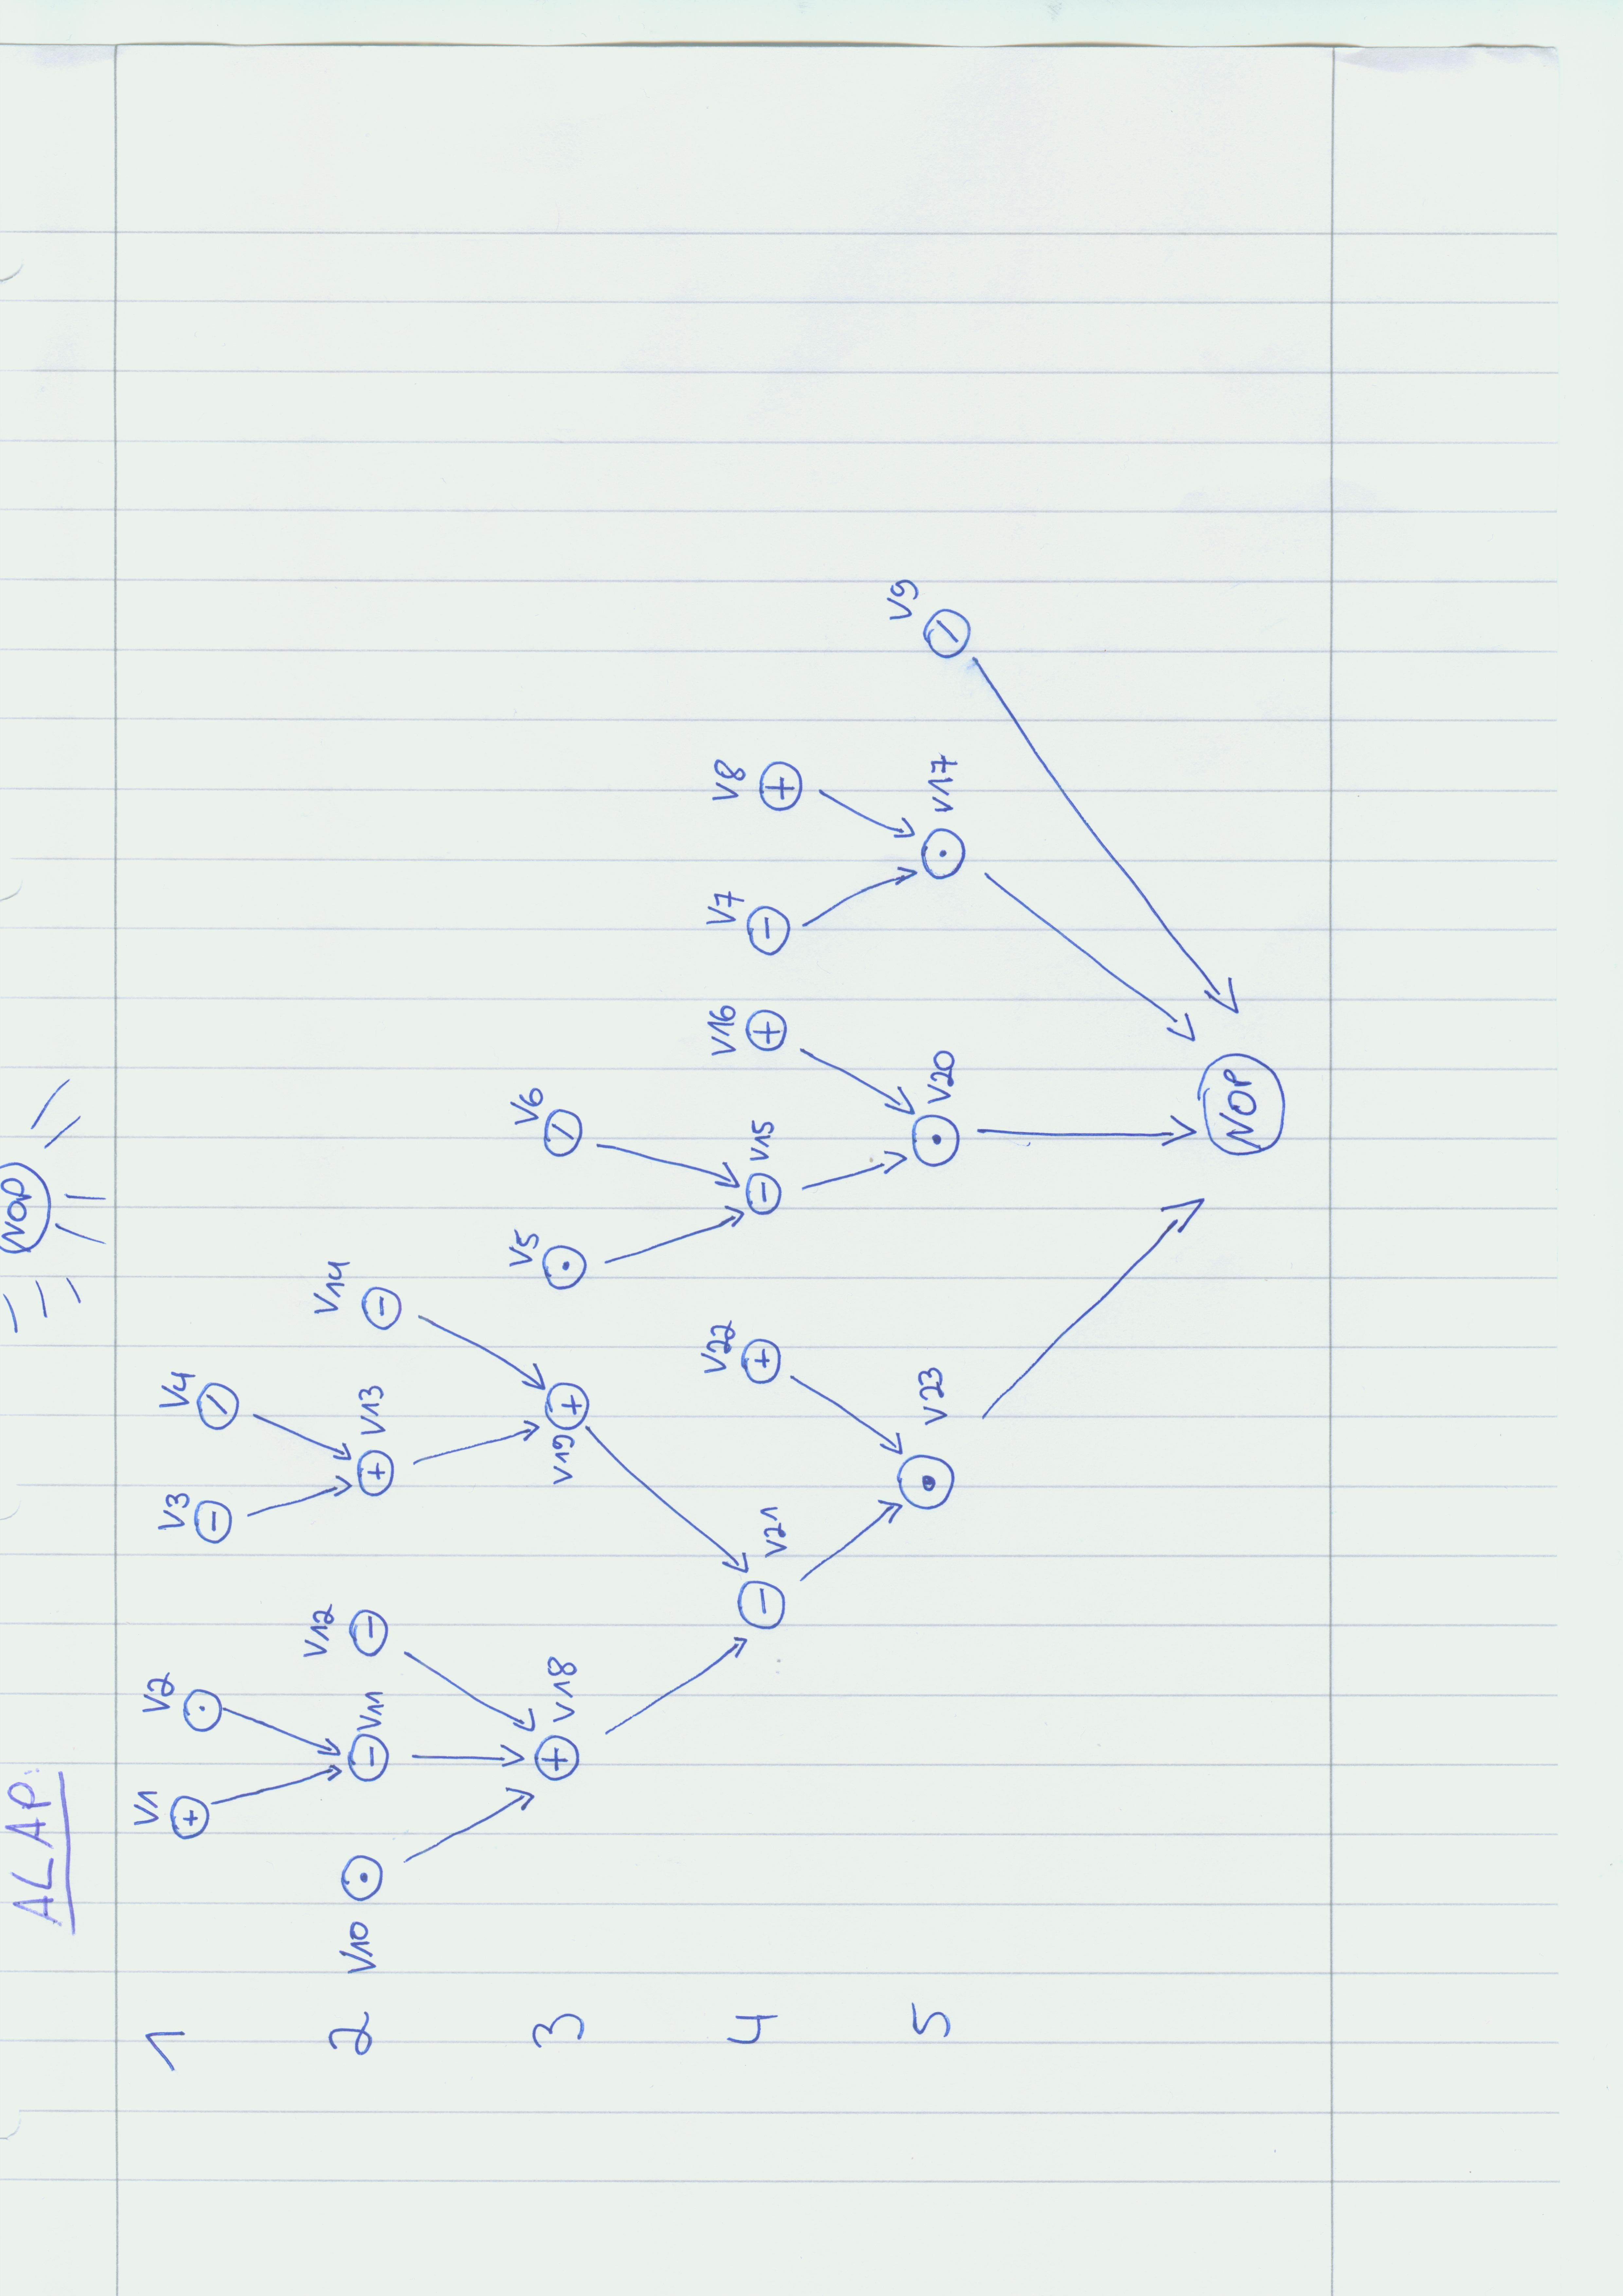
\includegraphics[scale=0.5, angle = -90]{Image125}
	
	\item
	
	Sequenzgraph mit Knotengewicht:
	
	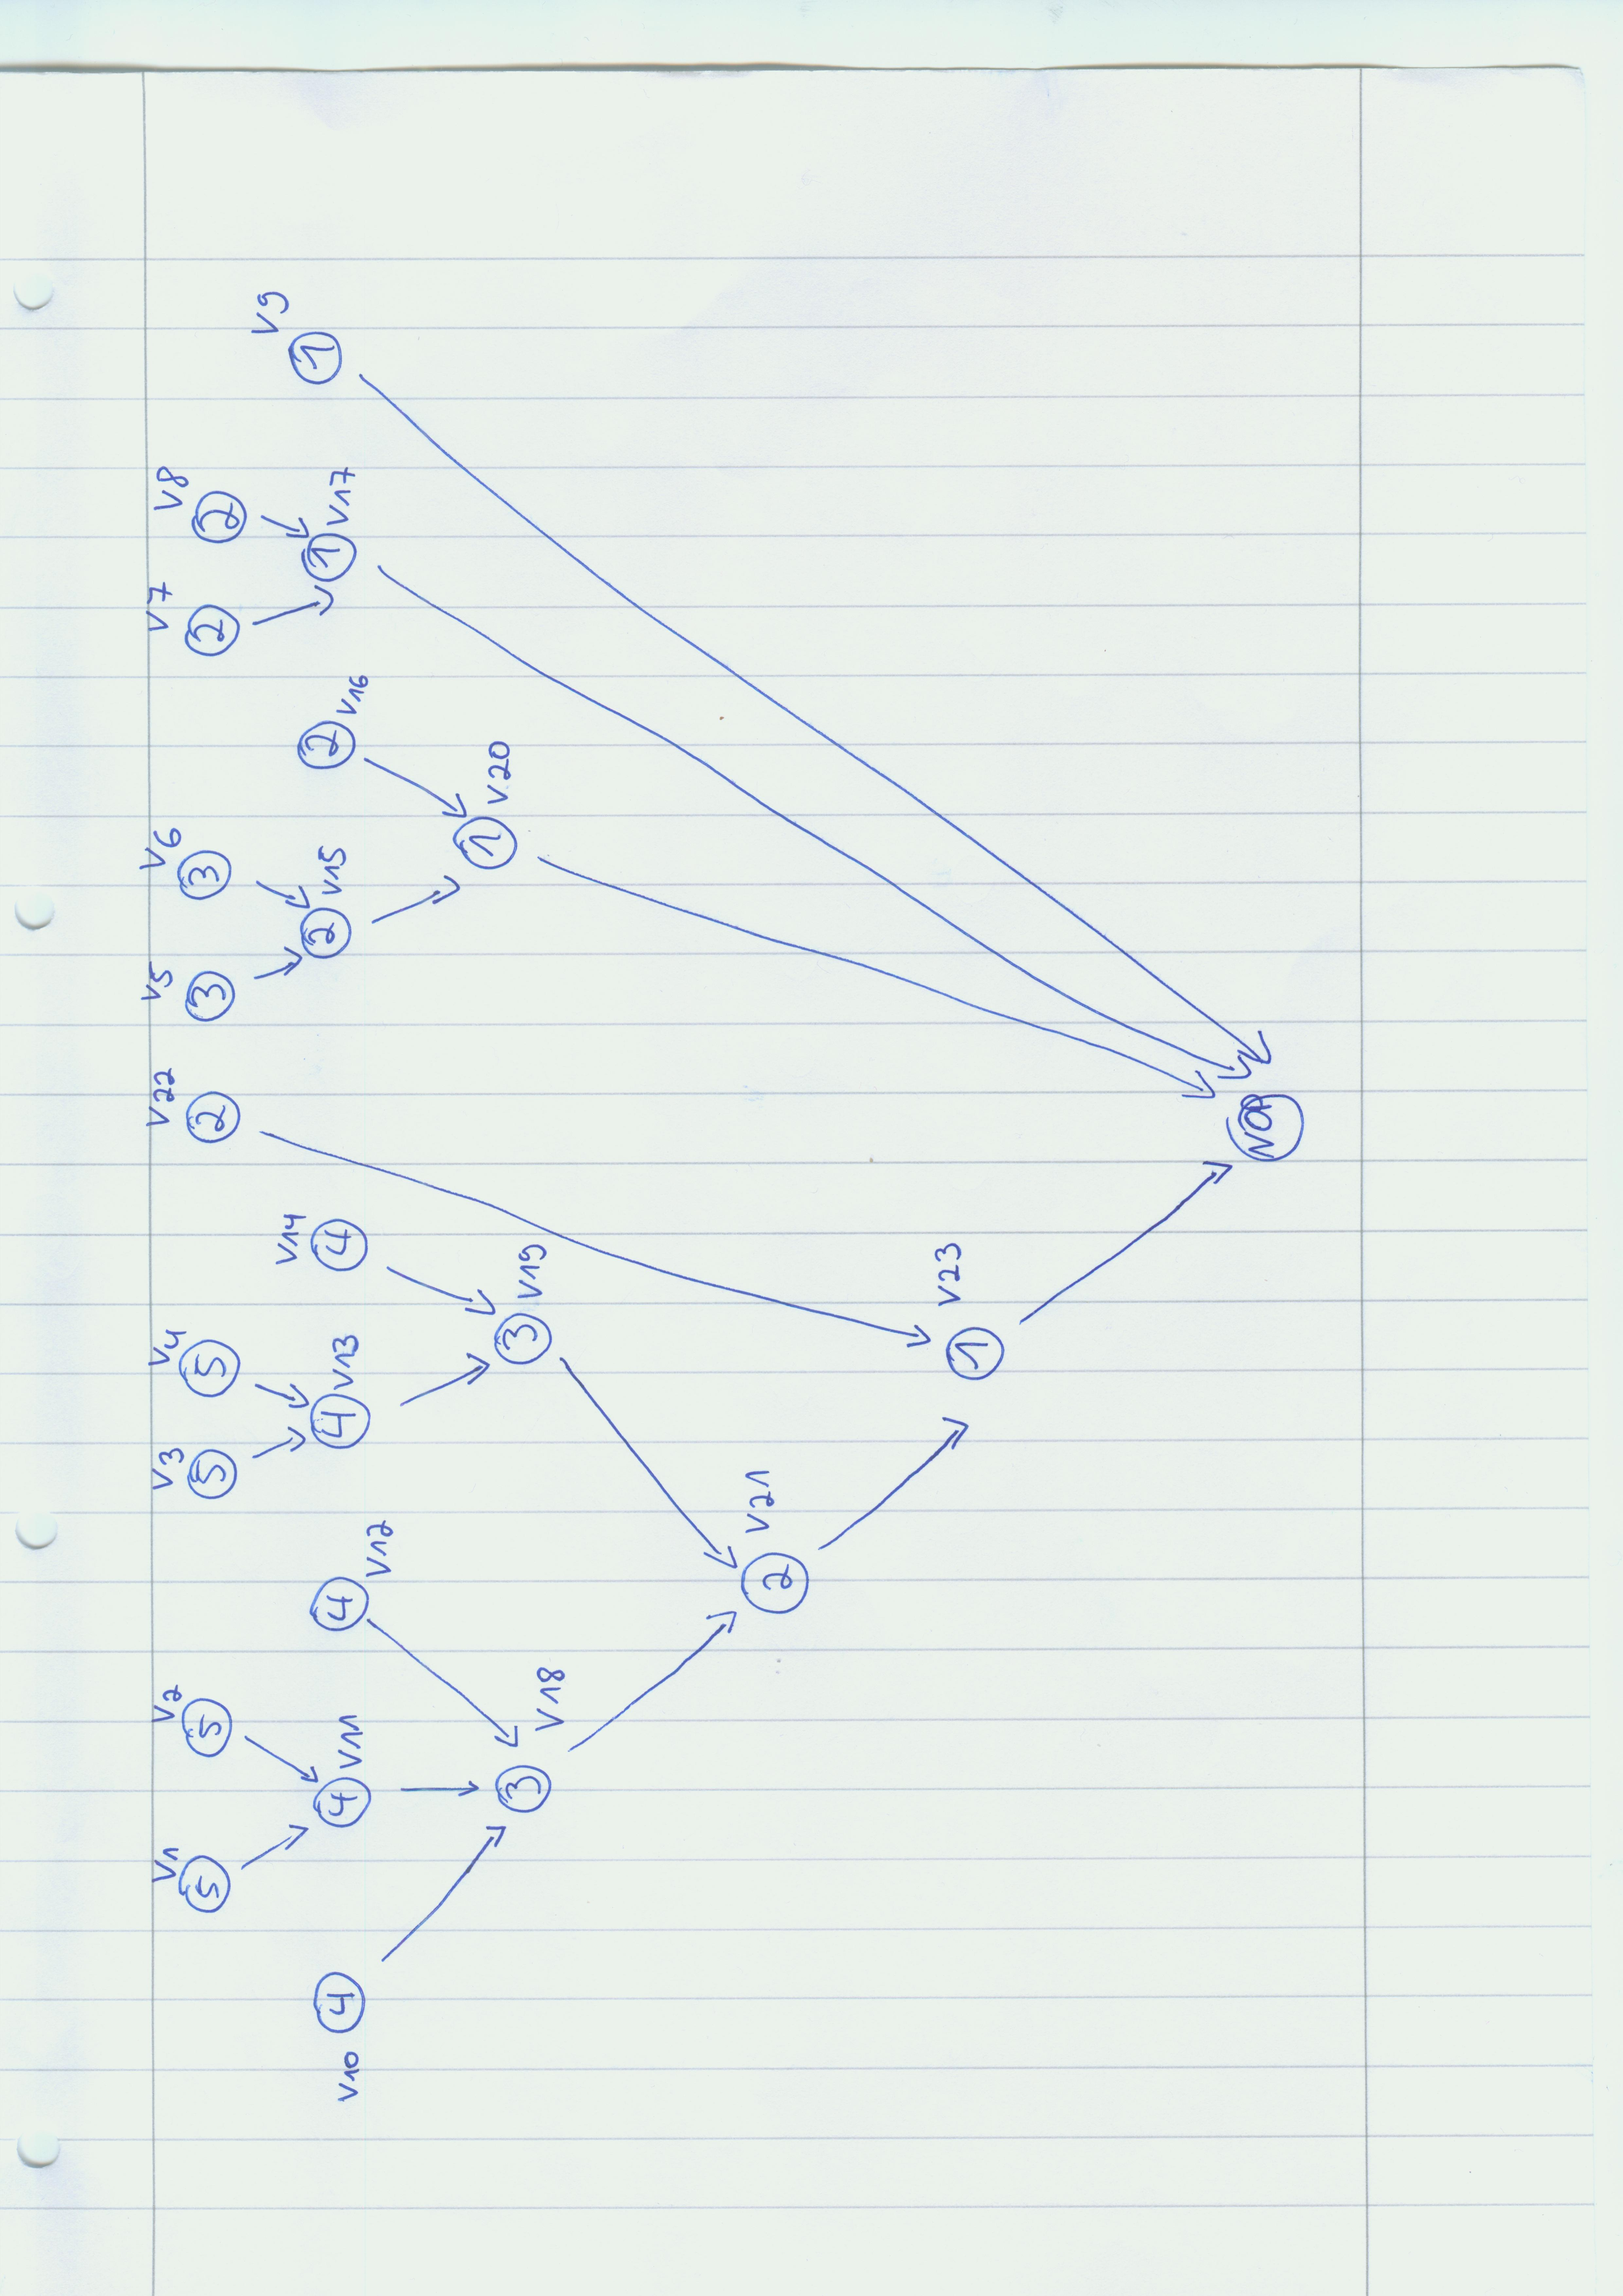
\includegraphics[scale=0.5, angle = -90]{Image126}
	\newpage
	Untere Schranke:
	
	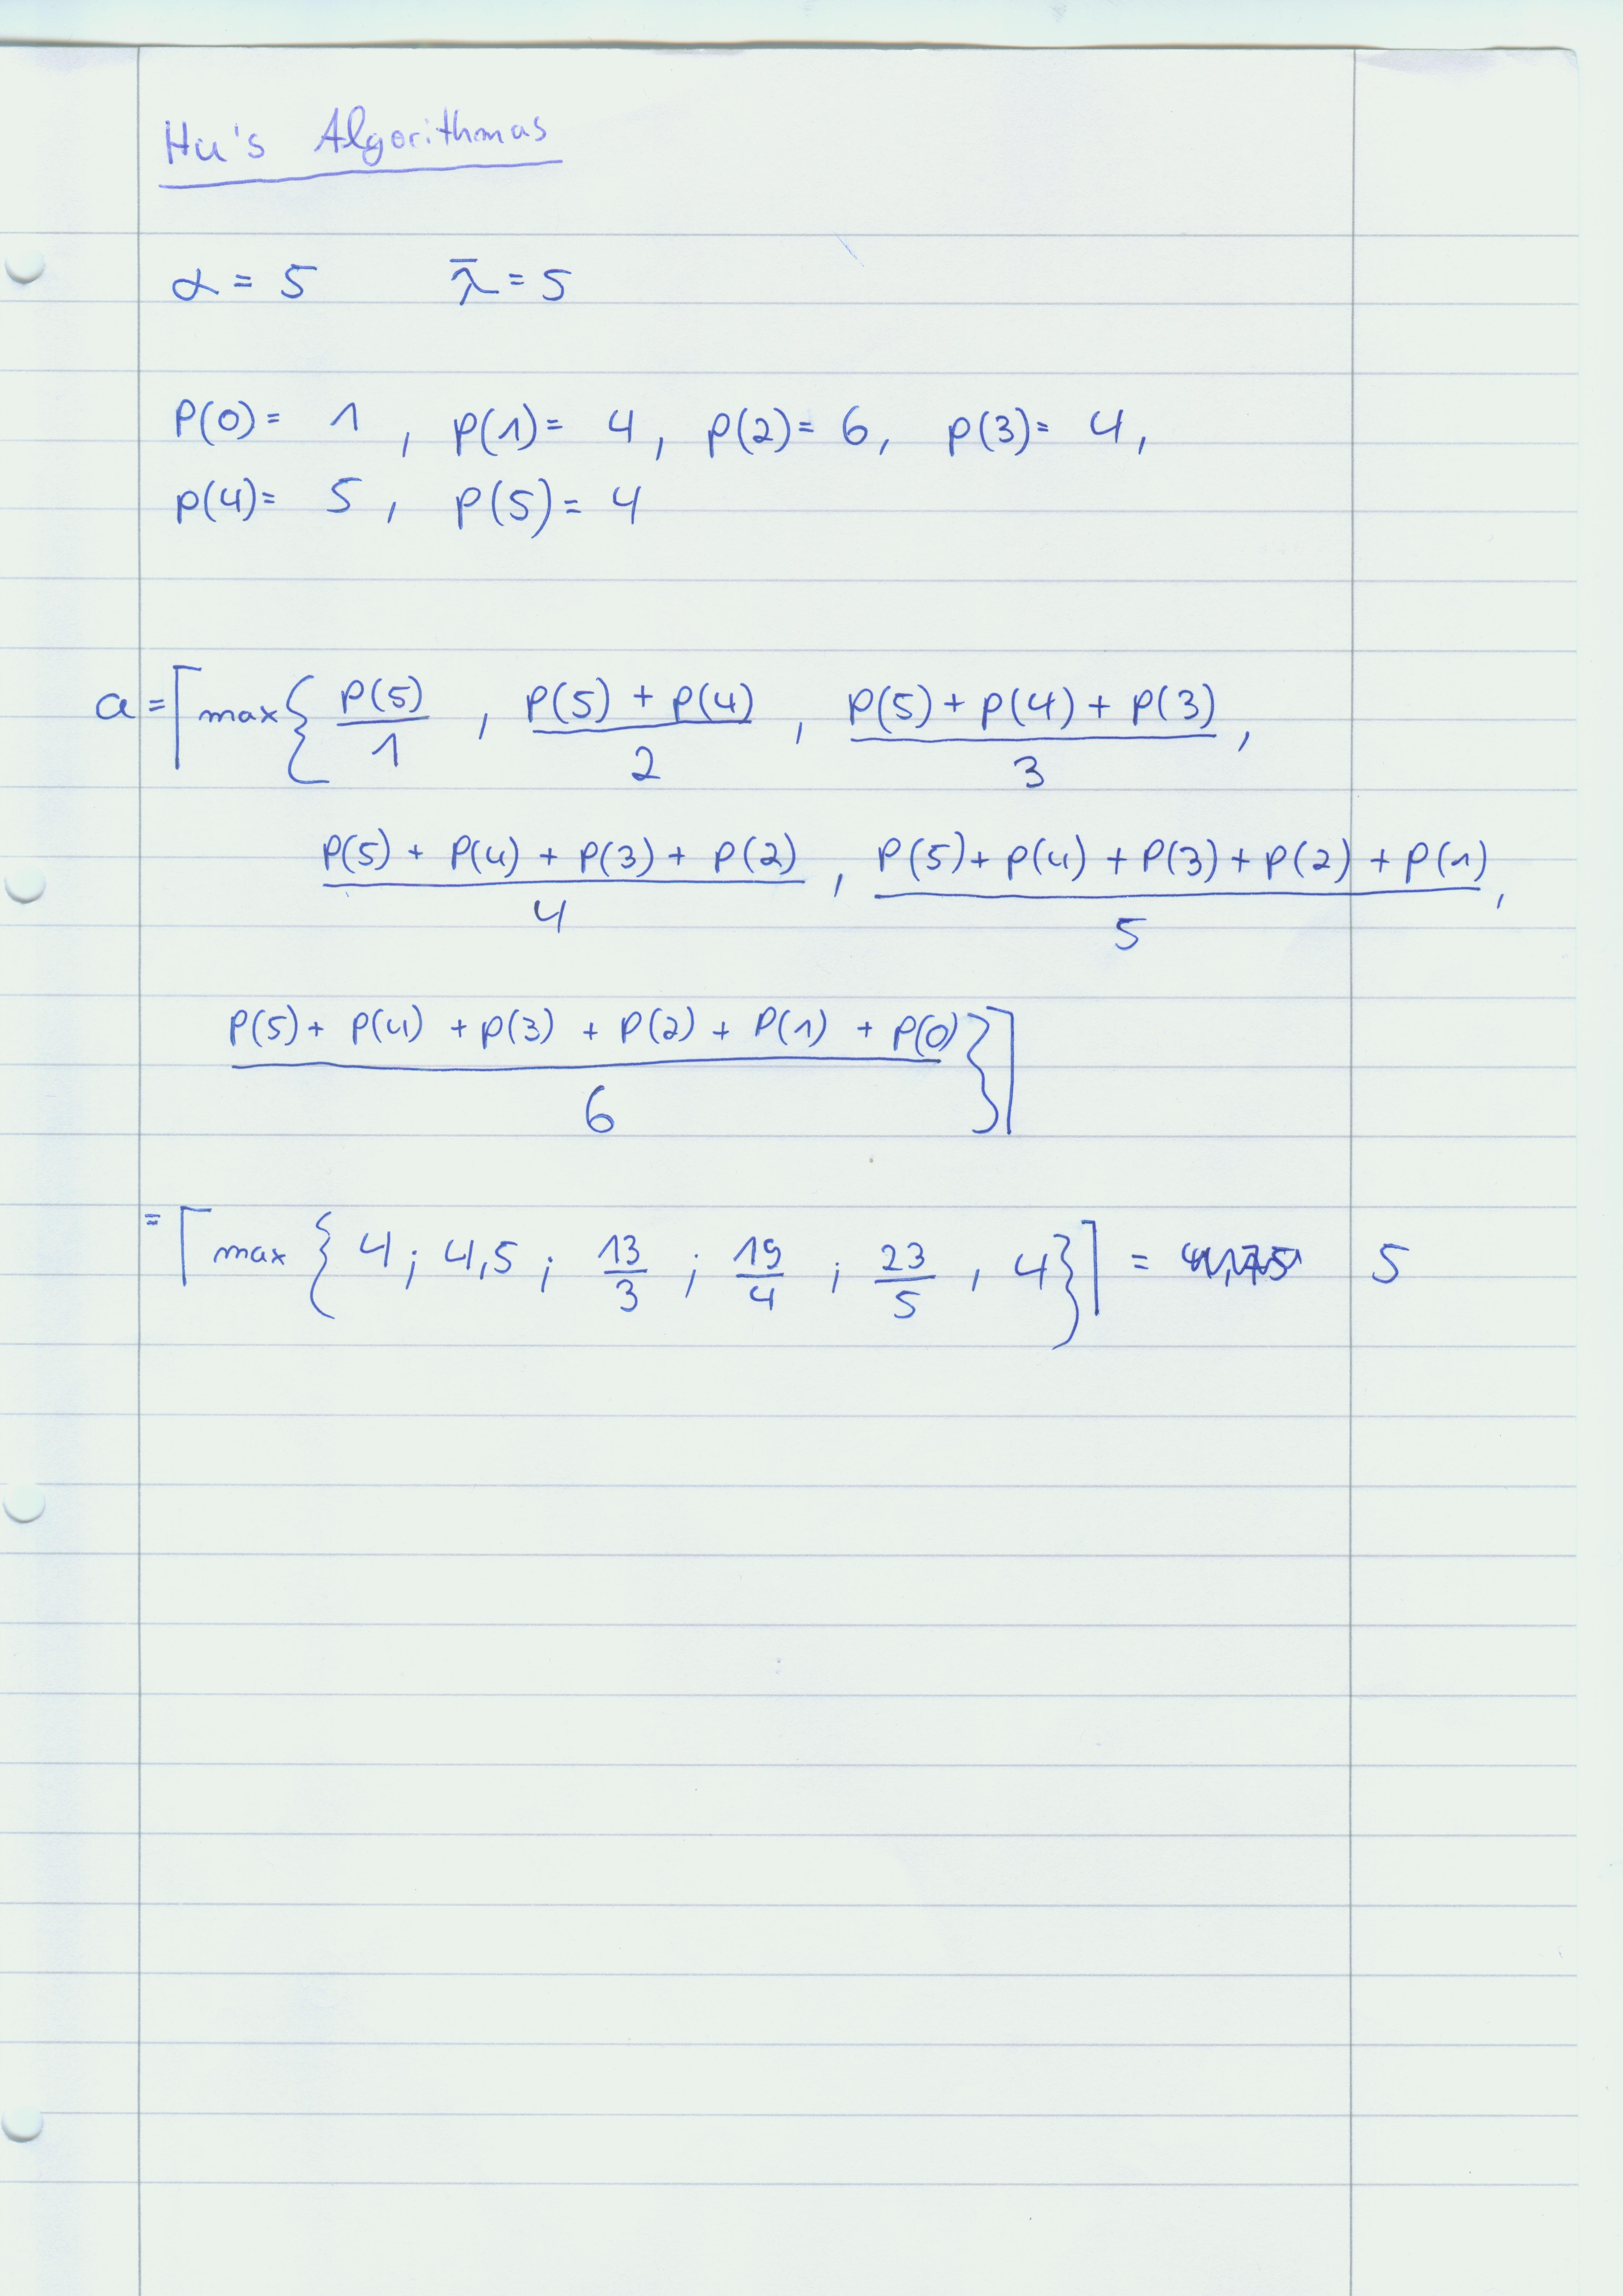
\includegraphics[width=1\textwidth]{Image127}
	\newpage
	Ablaufplan nach Hu:
	
	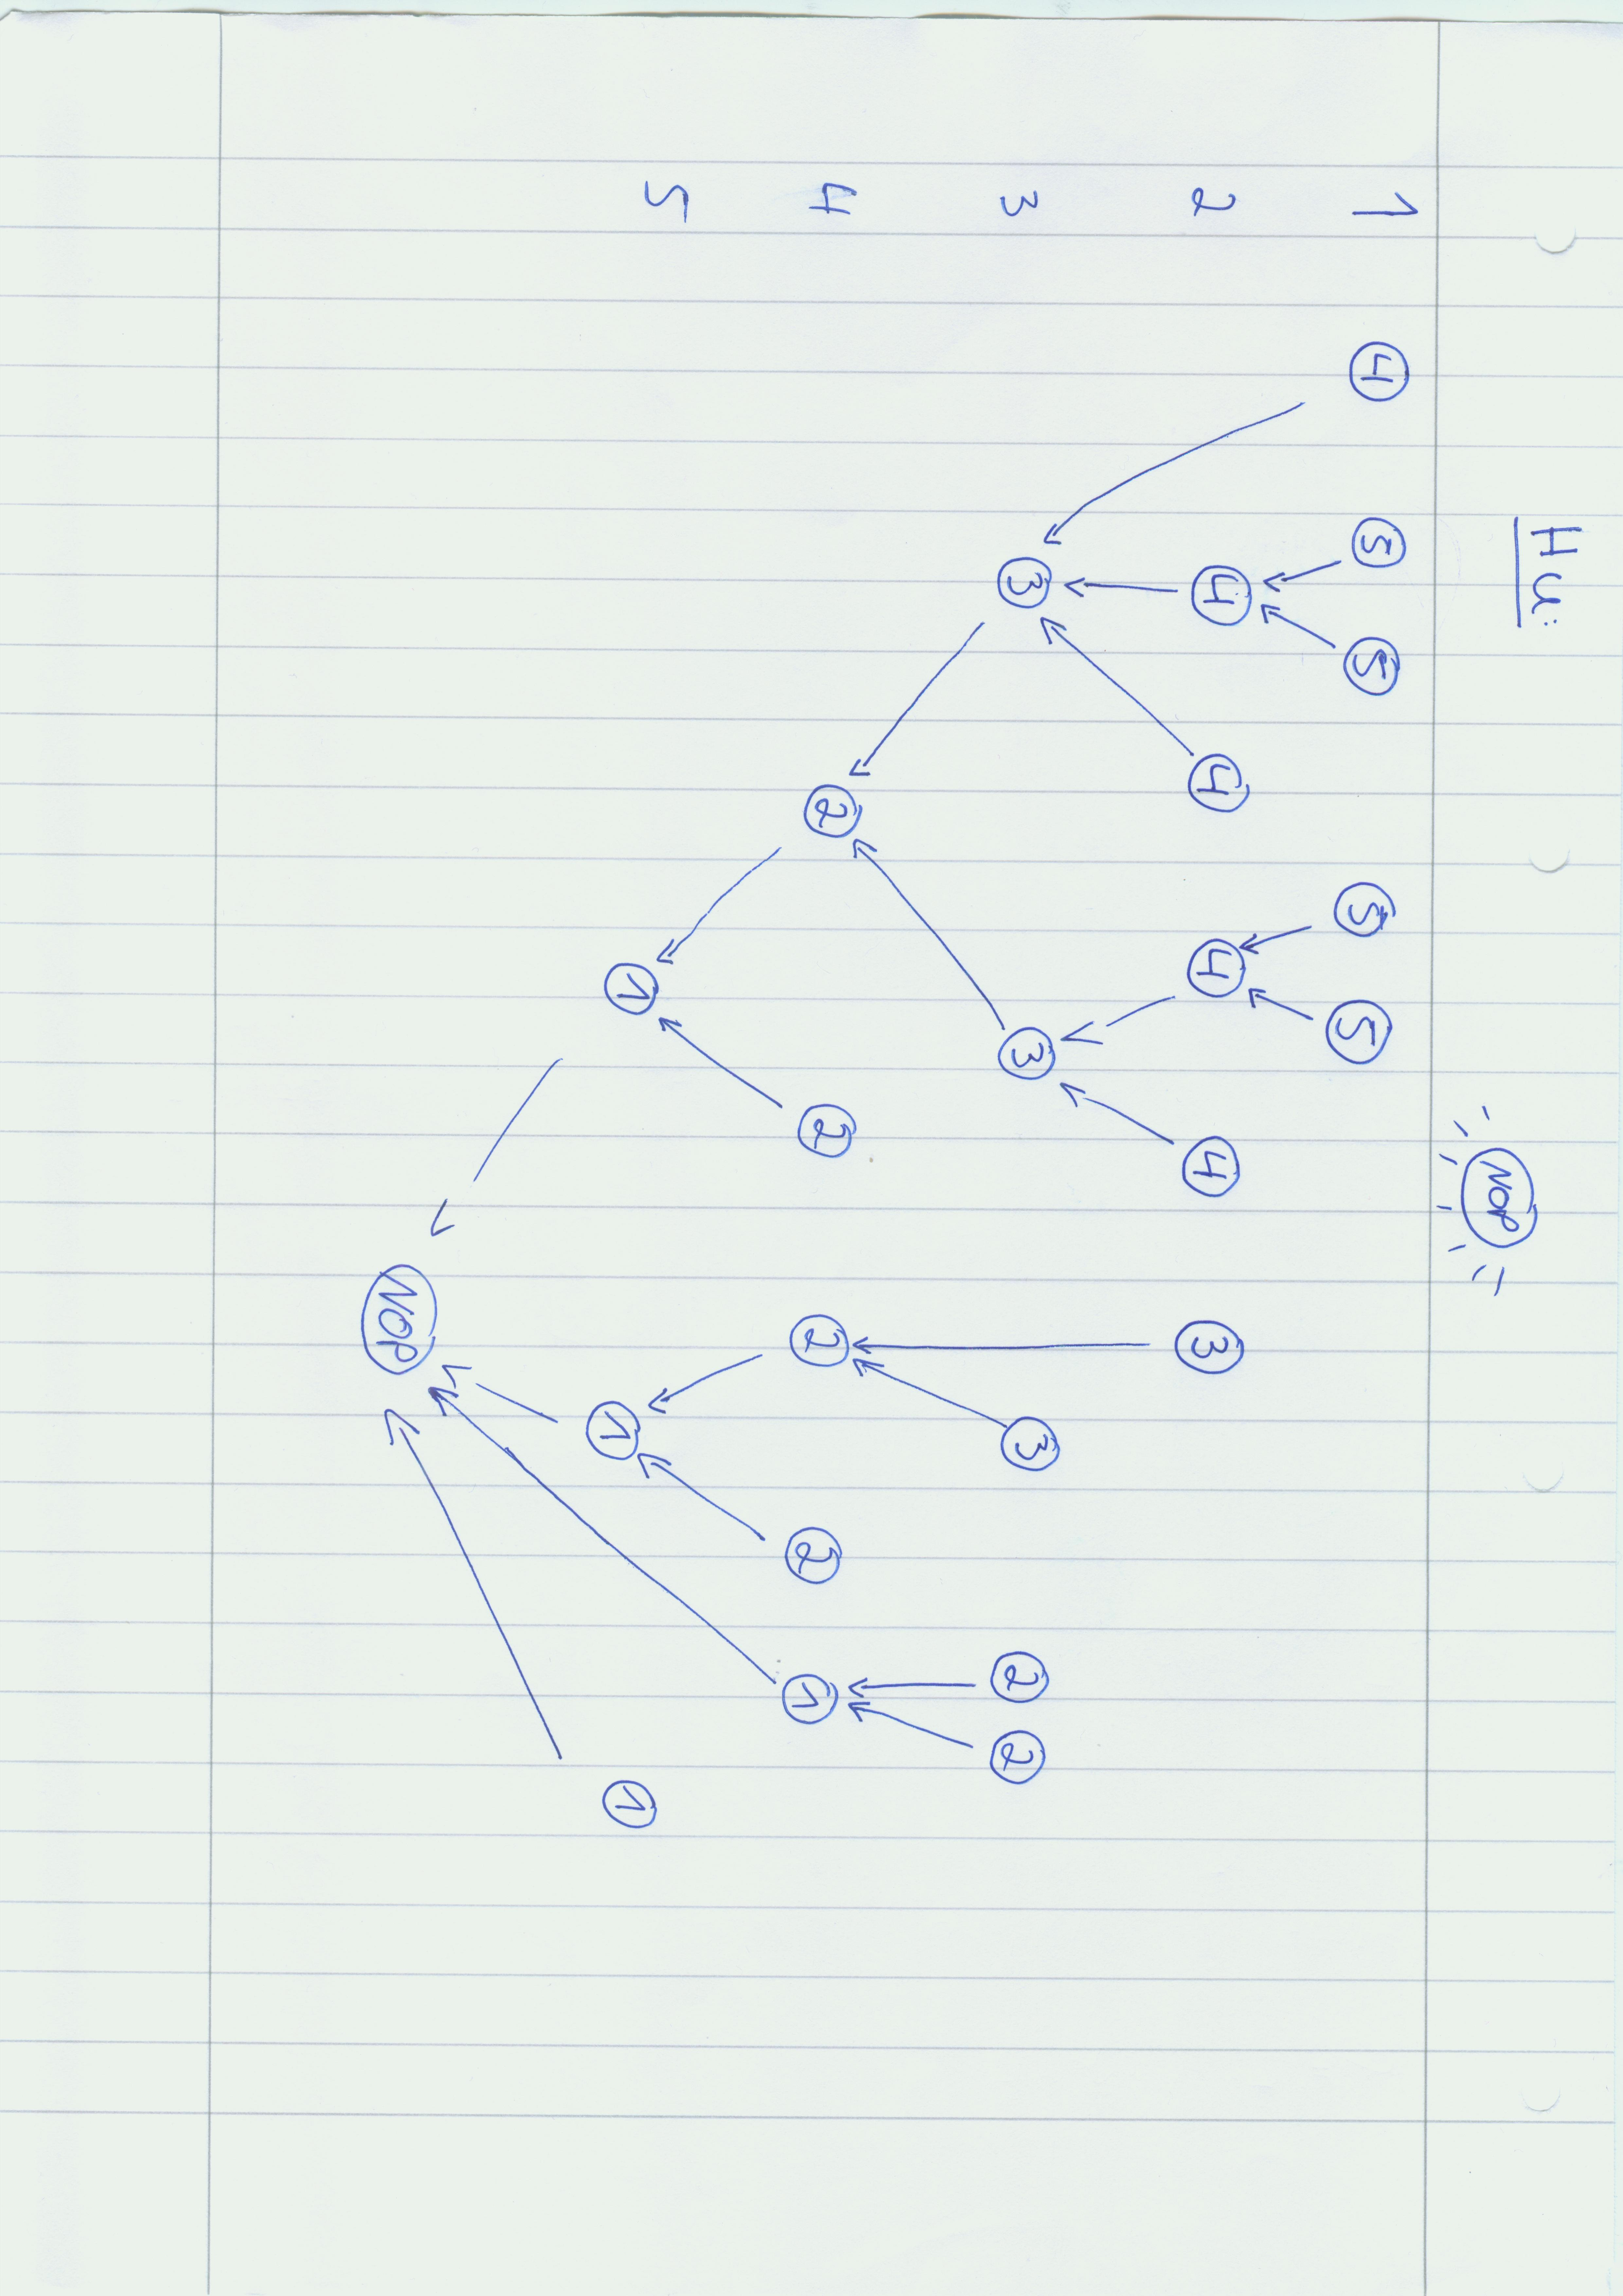
\includegraphics[scale=0.5, angle = 90]{Image128}
	
	\item \hfill
	
	\begin{tabular}{llll}
		& ASAP & ALAP & HU \\
		Fläche & 14 ALUS & 6 ALUS& 5 ALUS \\
		Latenz & 5 Takte & 5 Takte &  5 Takte\\		
	\end{tabular}
	
	Alle drei Scheduling Verfahren erzeugen ein Scheduling mit gleicher Latenz, die Fläche ist bei HUs Algorithmus allerdings am geringsten. Laut Foliensatz 07, S.37 erzeugt HUs Algorithmus ein Scheduling minimaler Latenz bei minimaler Fläche, wenn die Voraussetzungen, wie in diesem Beispiel, erfüllt sind. Es kann also kein Scheduling mit kleinerer Latenz geben.
	
	\item
	
	Listenbasierter Ablaufplan: \\
	Die hochgestellten Zahlen über den Knoten repräsentieren hier das Gewicht der Knoten, also die Anwendung der \glqq kritischer Pfad\grqq - Regel.
	
	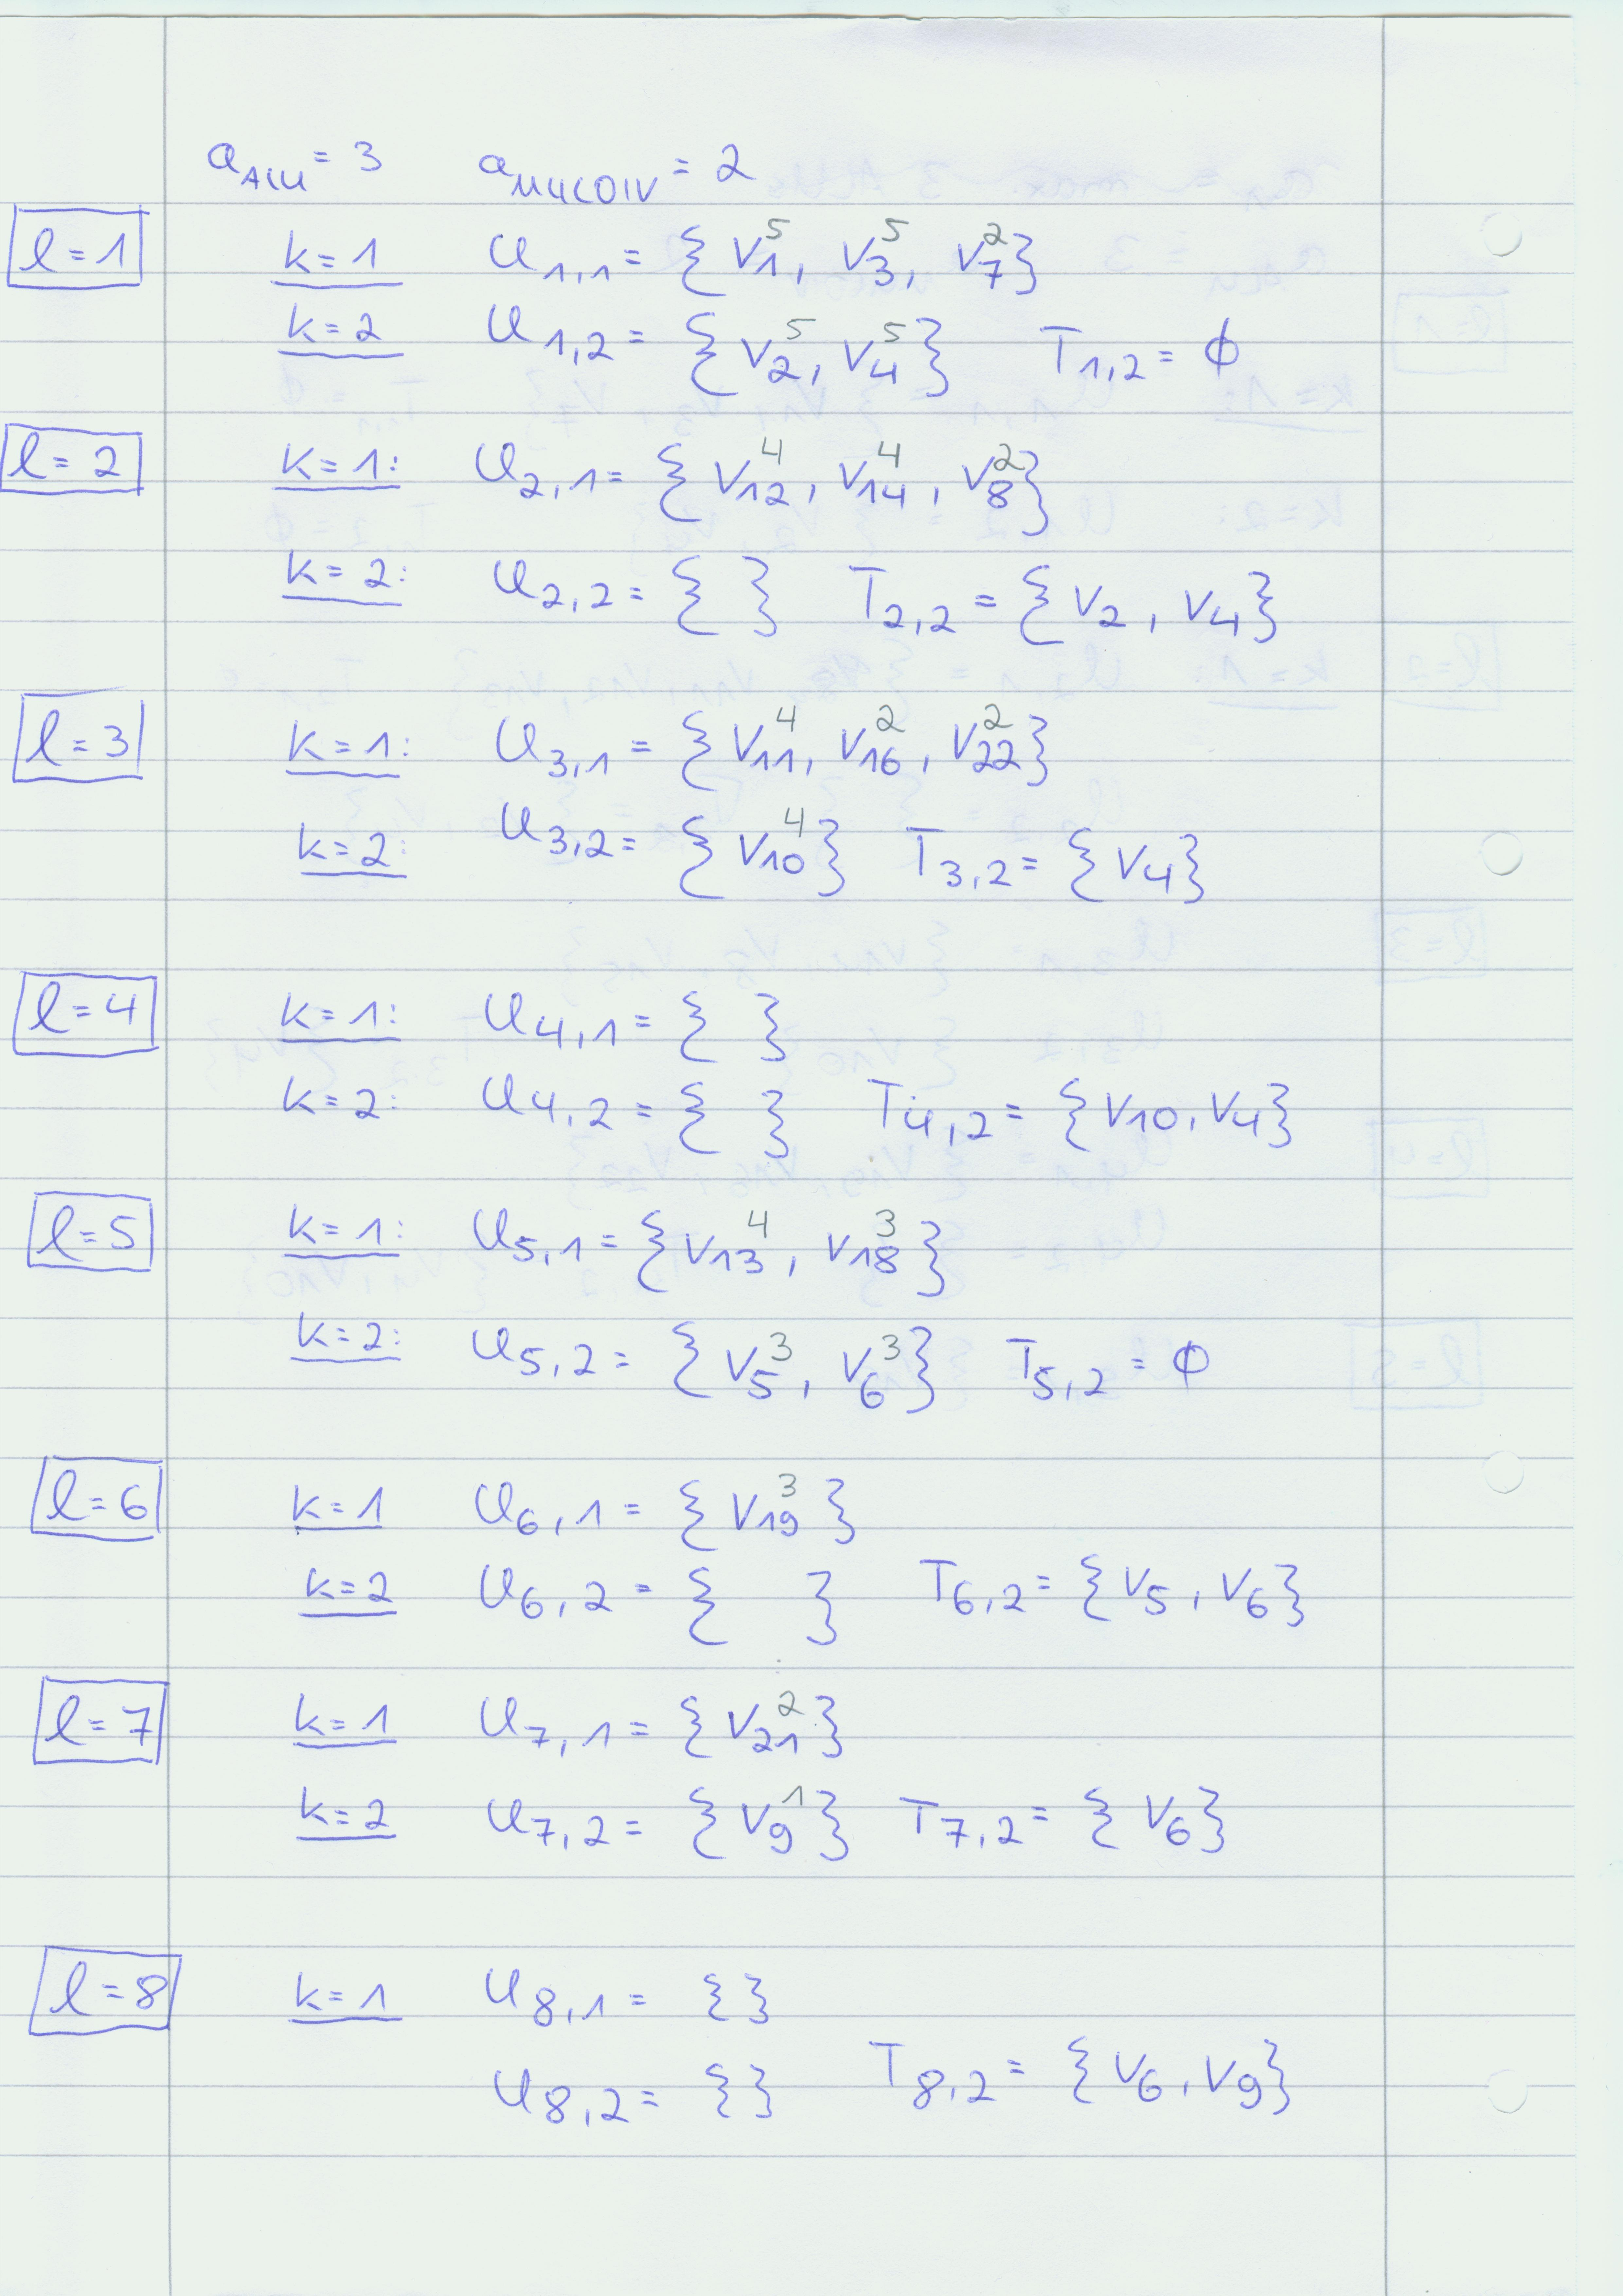
\includegraphics[scale=0.8]{Image129}
	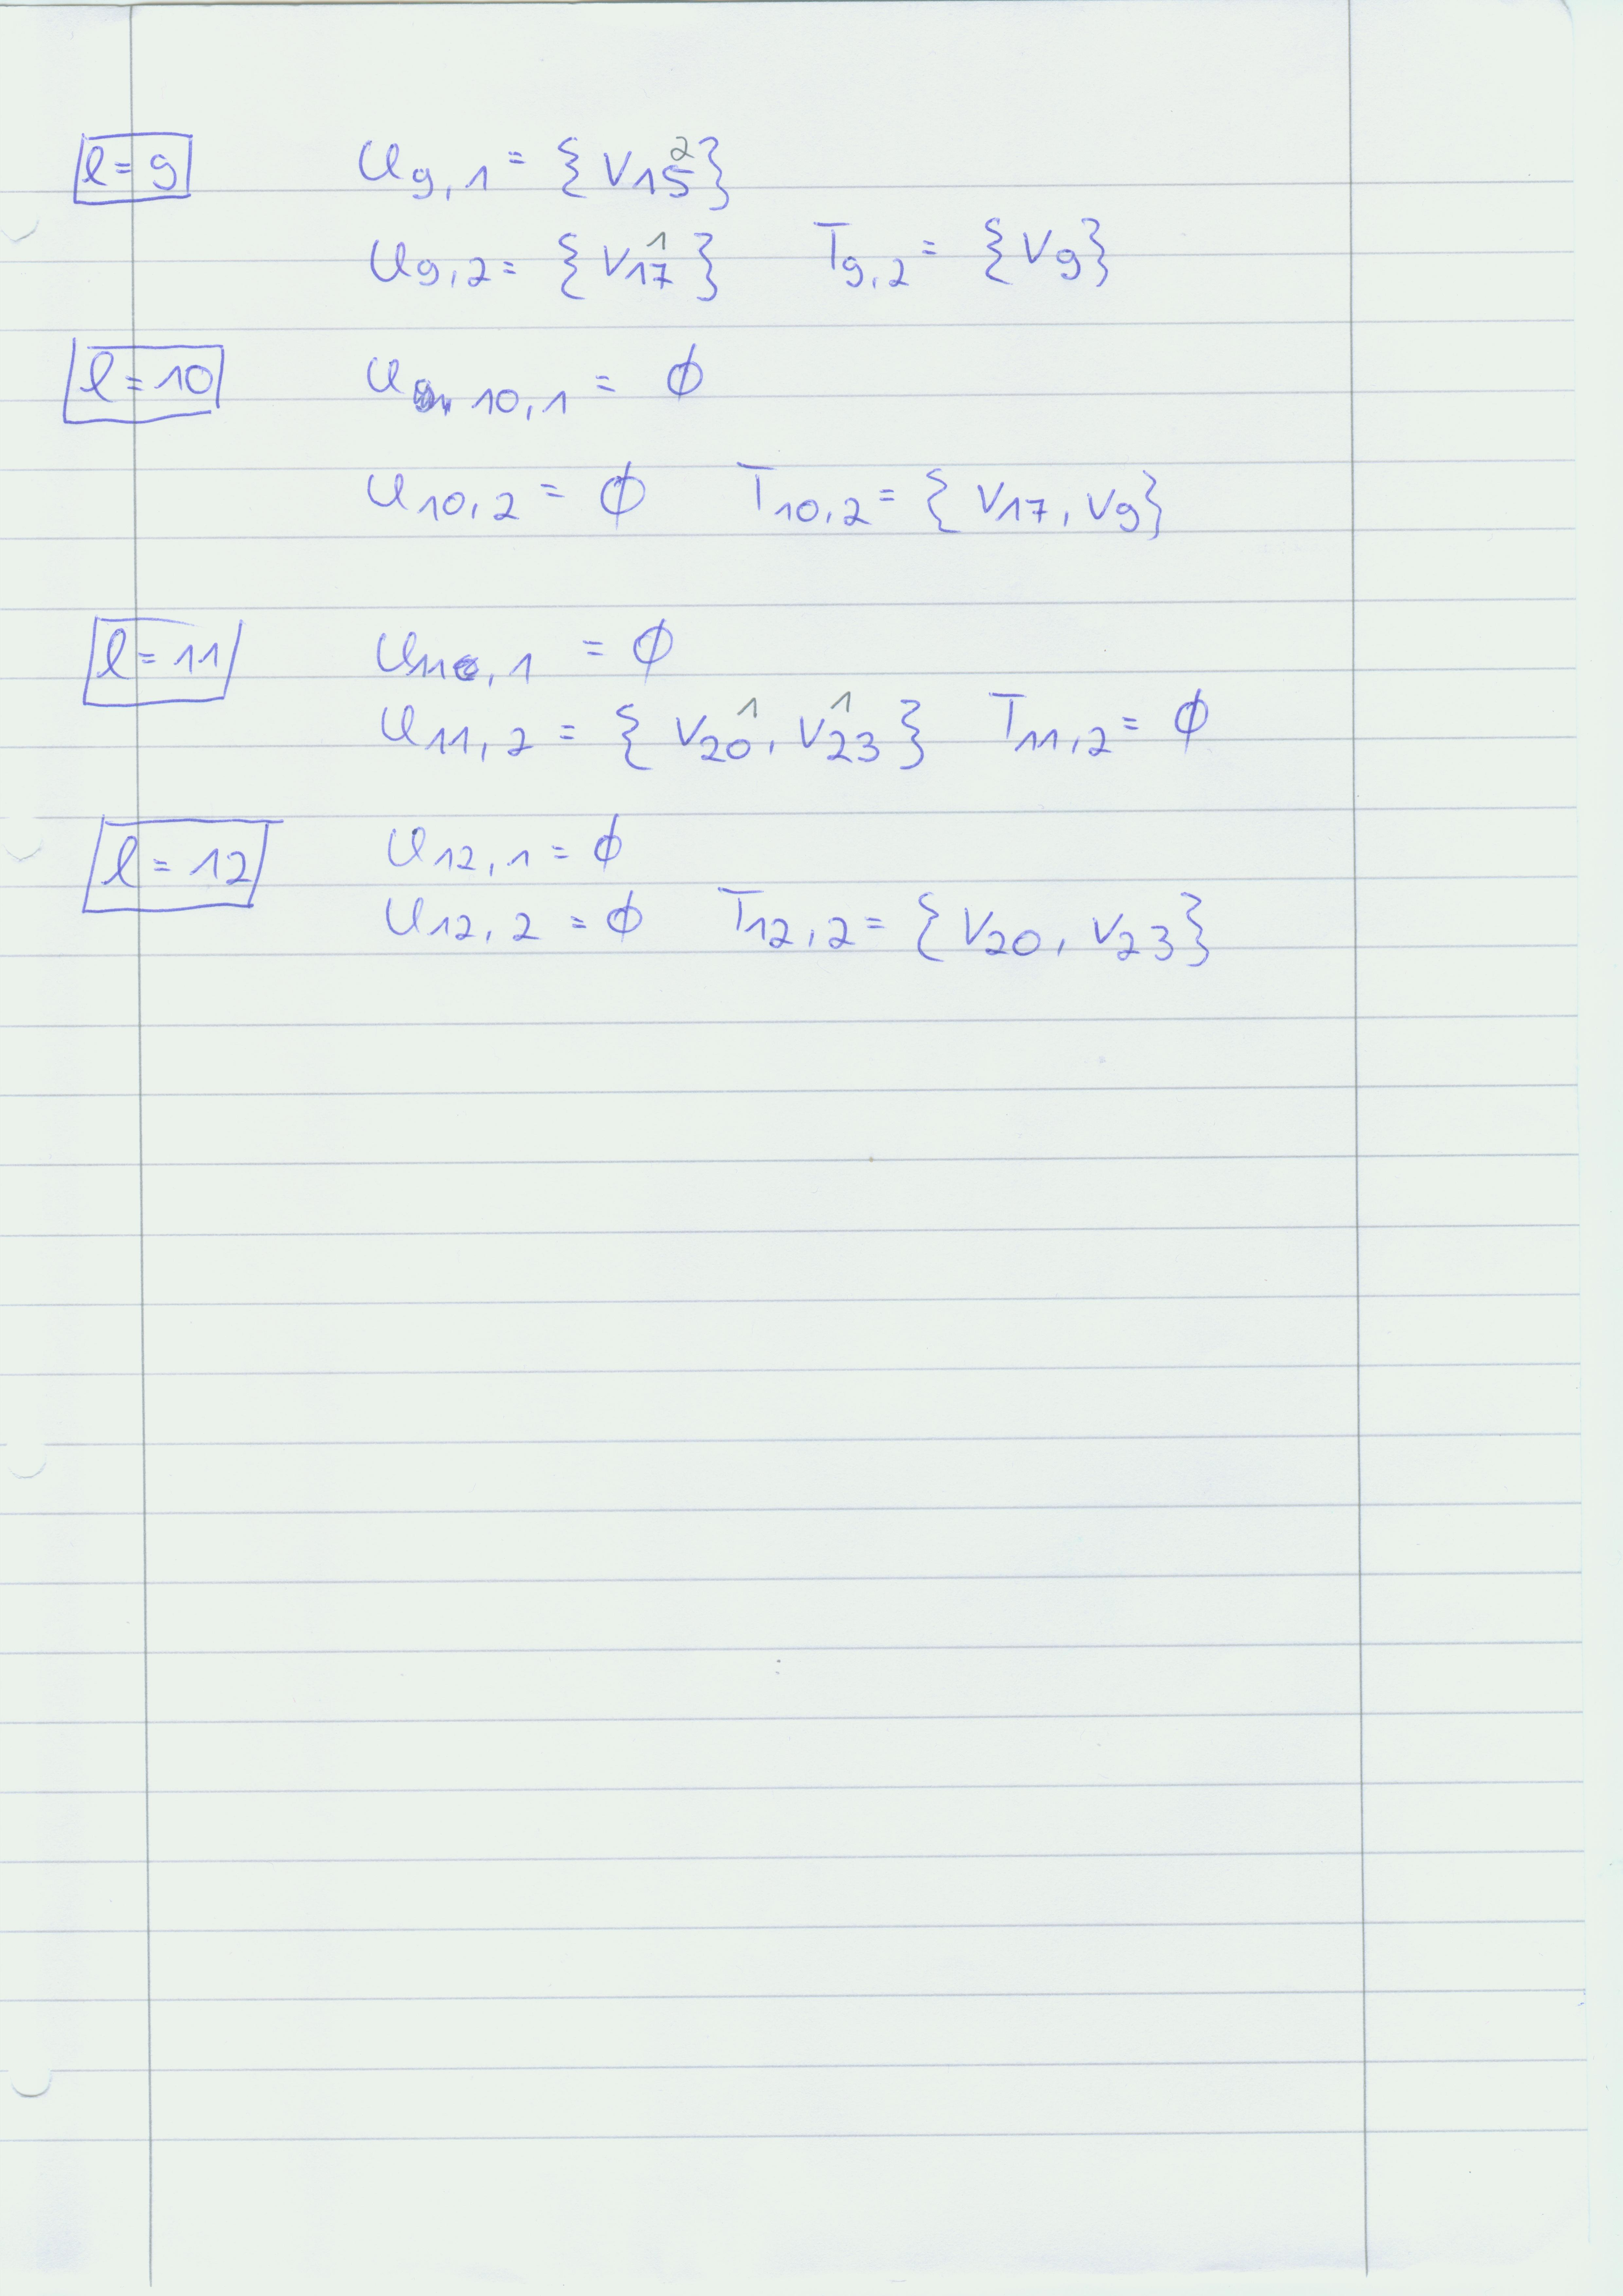
\includegraphics[scale=0.8]{Image130}
	
	Graphische Darstellung des Ablaufplans:
	
	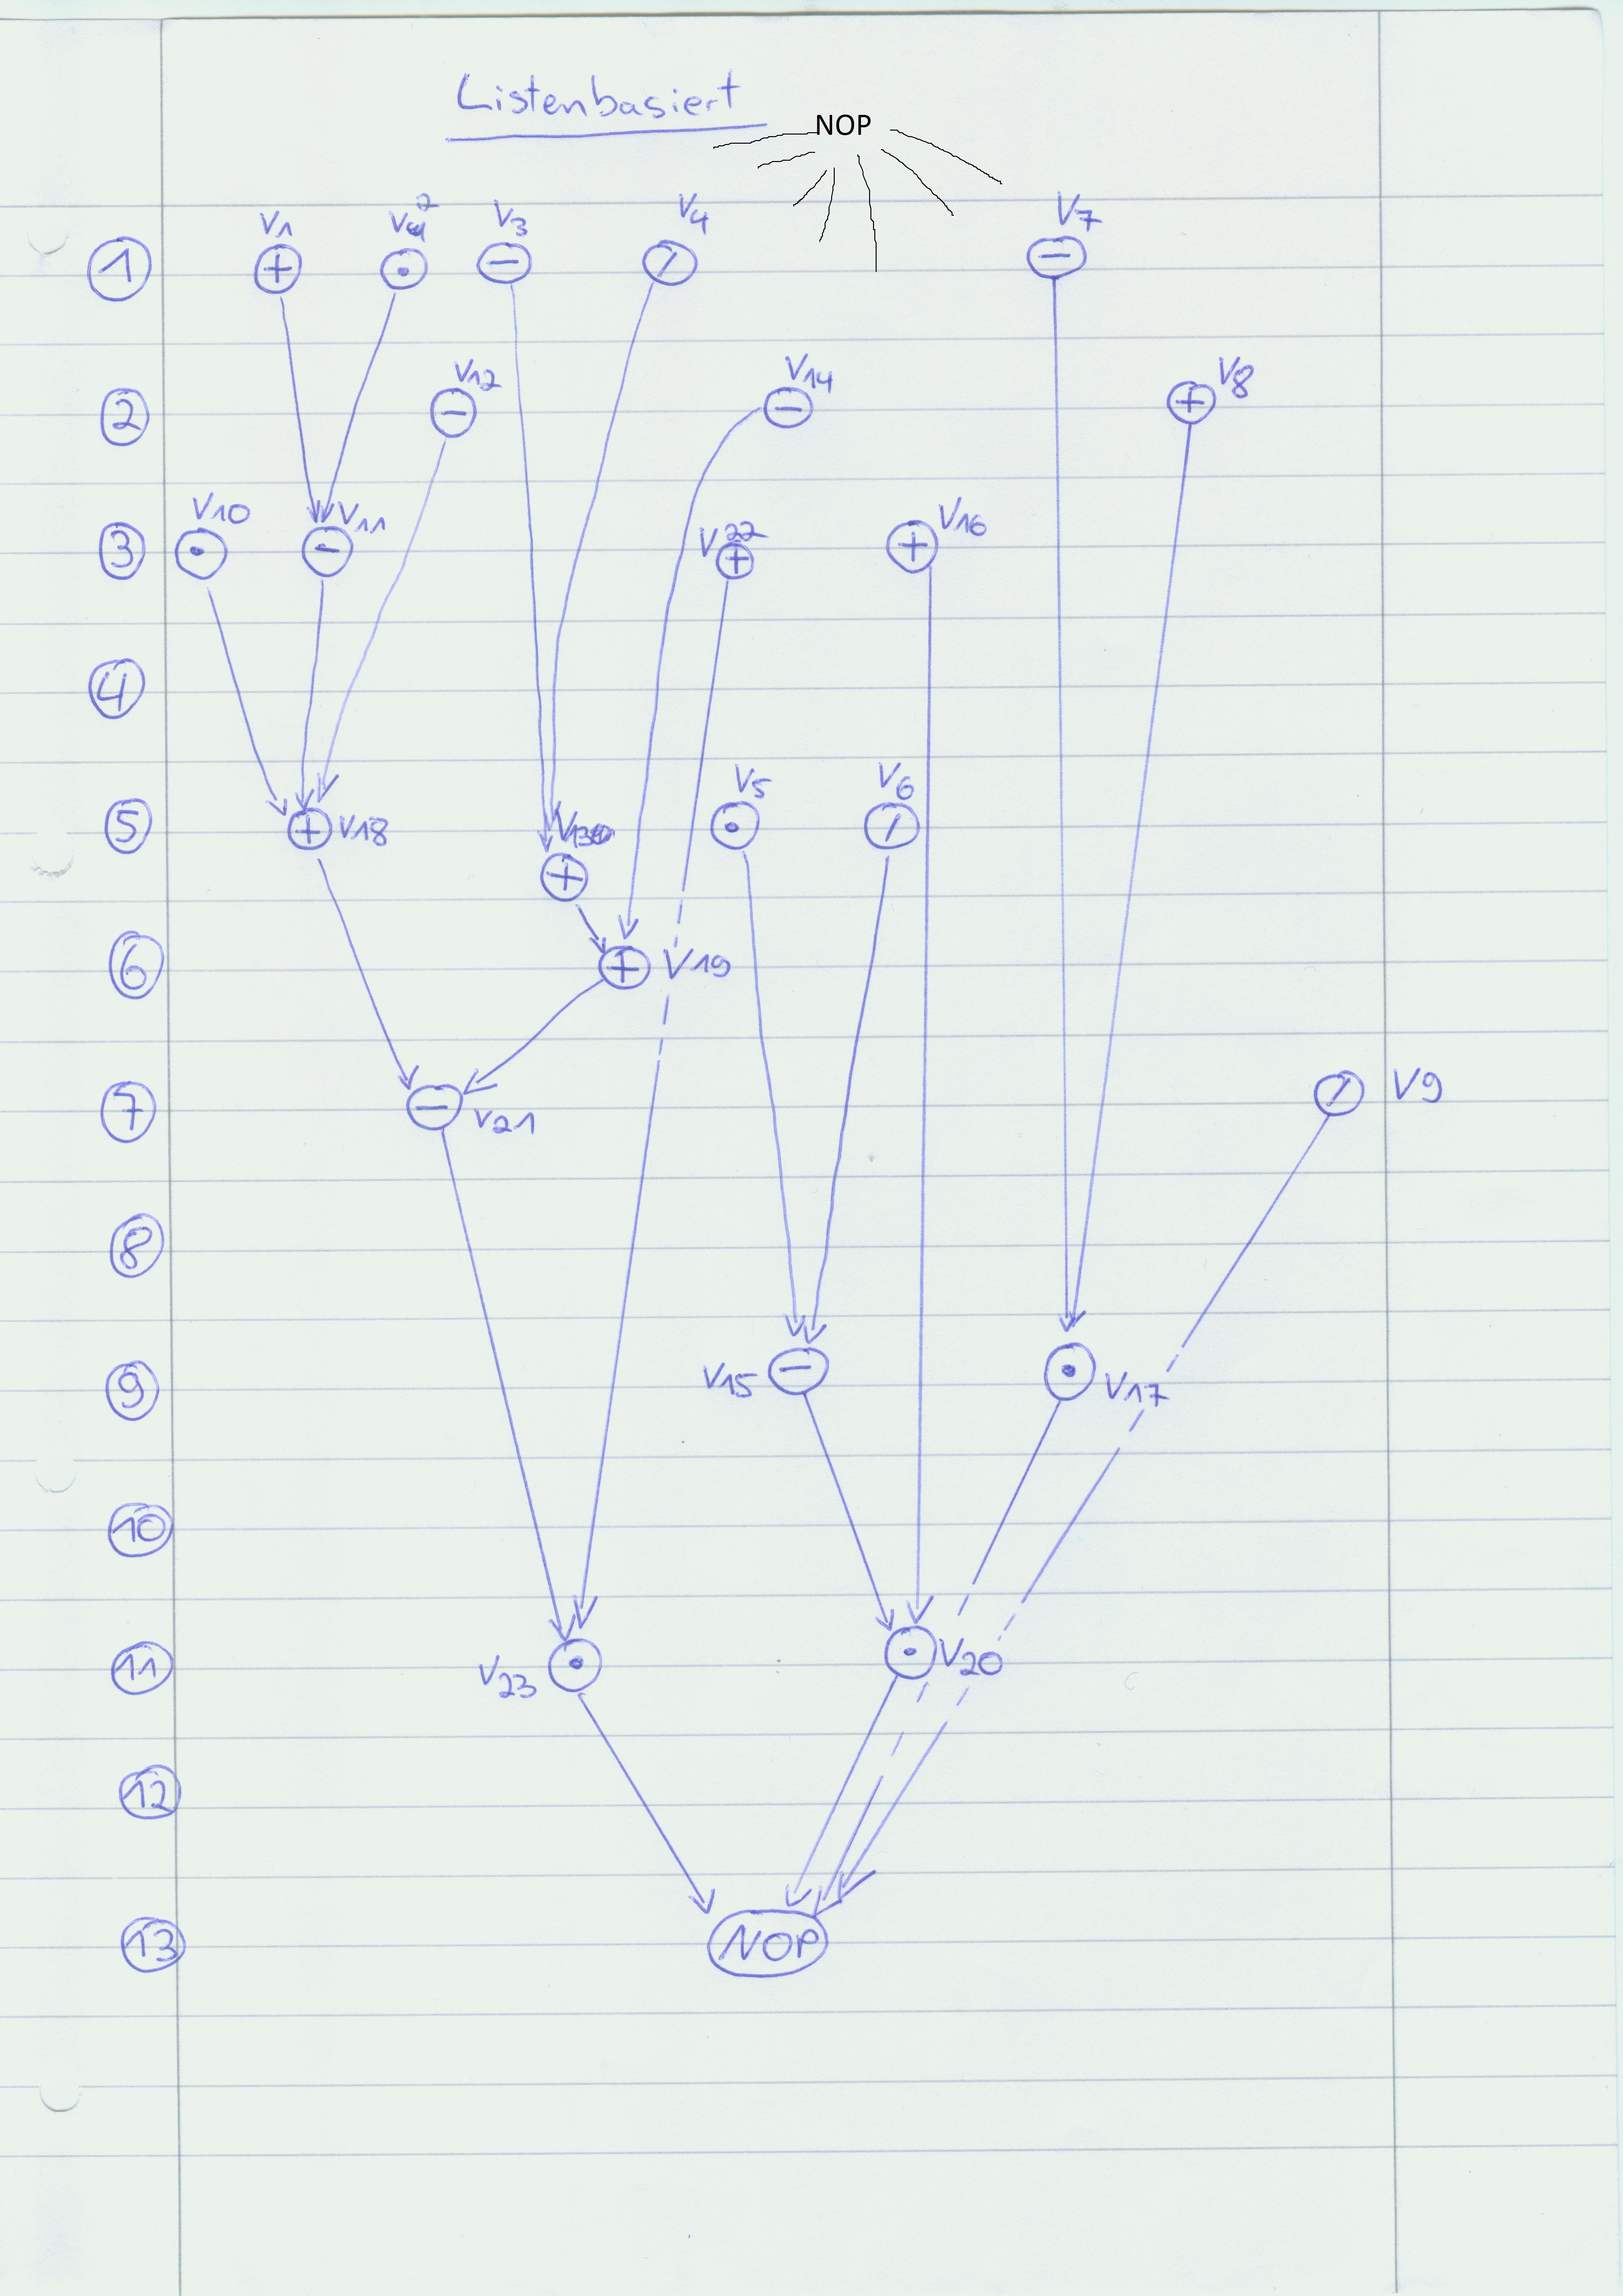
\includegraphics[scale=0.8]{Image131}
	
\end{enumerate}

\section*{Aufgabe 2: High Level Synthese: Force-Directed Scheduling}

\begin{enumerate}[(a)]
	\item Zeitrahmen:
	
	\begin{tabular}{|l||c|c|}
		\hline 
		Task& $t_i^L$ & $t_i^S$ \\ 
		\hline 
		1& 1 & 3 \\ 
		\hline 
		2& 1 & 4 \\ 
		\hline 
		3& 1 & 3 \\ 
		\hline 
		4& 2 & 4 \\ 
		\hline 
		5& 2 & 4 \\ 
		\hline 
		6& 3 & 5 \\ 
		\hline 
	\end{tabular} 
	
	Operations- und Operationstypwahrscheinlichkeiten:
	
	\begin{tabular}{|l||c|c|c|c|c|c|c|c|}
		\hline 
		Zeitschritt l& $p_1(l)$ & $p_2(l)$ & $p_3(l)$ & $p_4(l)$ & $p_5(l)$ & $p_6(l)$ & $q_{ALU}$ & $q_{MUL}$ \\ 
		\hline 
		1& 1/3 & 1/4 & 1/3 & 0   & 0   & 0   & 1/3 & 7/12 \\ 
		\hline 
		1& 1/3 & 1/4 & 1/3 & 1/3 & 1/3 & 0   & 2/3 & 11/12 \\ 
		\hline 
		1& 1/3 & 1/4 & 1/3 & 1/3 & 1/3 & 1/3 & 1   & 11/12 \\ 
		\hline 
		1& 0   & 1/4 & 0   & 1/3 & 1/3 & 1/3 & 2/3 & 7/12 \\ 
		\hline 
		1& 0   & 0   & 0   & 0   & 0   & 1/3 & 1/3 & 0 \\ 
		\hline 
	\end{tabular} 
	
	\item Selbstkräfte:
	
	Berechnung:\\
	Operationstypwahrscheinlichkeit $q_k(l)$\\
	Operationswahrscheinlichkeit $p_i(l)$\\
	Selbstkraft $F_{i,l}^{self} = q_k(l) - p_i(l) \sum_{m=t_i^S}^{t_i^S}q_k(m)$
	
	
	(ausführlich für v1, aus Platzgründen für den Rest nur das Ergebnis)
	
	\begin{tabular}{|c|c|c|c|c|c|c|}
		\hline 
		Zeitschritt l& $F_{1,l}^{self}$ & $F_{2,l}^{self}$ & $F_{3,l}^{self}$ & $F_{4,l}^{self}$ & $F_{5,l}^{self}$ & $F_{6,l}^{self}$ \\ 
		\hline 
		1& $\frac{1}{3}-\frac{1}{3}\cdot(\frac{1}{3}+\frac{2}{3}+1)=-\frac{1}{3}$ & $-\frac{2}{12}$ & $-\frac{2}{9}$ & $\frac{1}{3}$ & $\frac{7}{12}$ & $\frac{1}{3}$ \\ 
		\hline 
		2& $\frac{2}{3}-\frac{1}{3}\cdot(\frac{1}{3}+\frac{2}{3}+1)=0$ & $\frac{2}{12}$ & $\frac{1}{18}$ & $-\frac{1}{9}$ & $\frac{1}{18}$ & $\frac{2}{3}$ \\ 
		\hline 
		3& $1-\frac{1}{3}\cdot(\frac{1}{3}+\frac{2}{3}+1)=\frac{1}{3}$ & $\frac{2}{12}$ & $\frac{1}{18}$ & $\frac{2}{9}$ & $\frac{1}{18}$ & $\frac{1}{3}$ \\ 
		\hline 
		4& $\frac{2}{3}-0=\frac{2}{3}$ & $-\frac{2}{12}$ & $\frac{7}{12}$ & $-\frac{1}{9}$ & $-\frac{2}{9}$ & 0 \\ 
		\hline 
		5& $\frac{1}{3}-0=\frac{1}{3}$ & 0 & 0 & $\frac{1}{3}$ & 0 & $-\frac{1}{3}$ \\ 
		\hline 
	\end{tabular} 
	\item Wir schedulen den Task mit der kleinsten Gesamtkraft. Für die Gesamtkraft addieren wir die Predecessor- und Successorkräfte auf die Selbstkräfte. In diesem Fall haben sowohl Operation 1 in Zeitschritt 1 als auch Operation 6 in Zeitschritt 5 eine minimale Gesamtkraft von $-\frac{1}{3}$.\\
	Damit würden wir Task 1 in Takt 1 starten, ebensogut könnte man auch Task 6 in Takt 5 starten
	\item Die Optimierung der Fläche unter Zeitconstraints geschieht beim kräftebasierten Schedulingansatz durch Auswahl des Tasks mit der \textbf{kleinsten} Gesamtkraft.\\
	Bei der Optimierung der Latenz unter Flächenconstraints wird der Force Directed List Schdeduling Algorithmus genutzt, bei dem die Selektionsprozedur kräftegesteuert ist. Hier wird jedoch der Task mit der \textbf{größten} Kraft ausgewählt, da wir die gegebenen Ressourcen möglichst gut auslasten wollen, um nicht unnötige Latenzen zu erhalten.
\end{enumerate}

	
\end{document}

